%2multibyte Version: 5.50.0.2953 CodePage: 1252

\documentclass{article}
%%%%%%%%%%%%%%%%%%%%%%%%%%%%%%%%%%%%%%%%%%%%%%%%%%%%%%%%%%%%%%%%%%%%%%%%%%%%%%%%%%%%%%%%%%%%%%%%%%%%%%%%%%%%%%%%%%%%%%%%%%%%%%%%%%%%%%%%%%%%%%%%%%%%%%%%%%%%%%%%%%%%%%%%%%%%%%%%%%%%%%%%%%%%%%%%%%%%%%%%%%%%%%%%%%%%%%%%%%%%%%%%%%%%%%%%%%%%%%%%%%%%%%%%%%%%
\usepackage{amsfonts}
\usepackage{amsmath}

\setcounter{MaxMatrixCols}{10}
%TCIDATA{OutputFilter=LATEX.DLL}
%TCIDATA{Version=5.50.0.2953}
%TCIDATA{Codepage=1252}
%TCIDATA{<META NAME="SaveForMode" CONTENT="1">}
%TCIDATA{BibliographyScheme=Manual}
%TCIDATA{Created=Tuesday, September 13, 2016 11:26:35}
%TCIDATA{LastRevised=Tuesday, October 15, 2019 14:55:43}
%TCIDATA{<META NAME="GraphicsSave" CONTENT="32">}
%TCIDATA{<META NAME="DocumentShell" CONTENT="Standard LaTeX\Blank - Standard LaTeX Article">}
%TCIDATA{CSTFile=40 LaTeX article.cst}
\usepackage{enumitem}
\usepackage{floatrow}
\usepackage{graphicx} 
\usepackage{caption}

\newtheorem{theorem}{Theorem}
\newtheorem{acknowledgement}[theorem]{Acknowledgement}
\newtheorem{algorithm}[theorem]{Algorithm}
\newtheorem{axiom}[theorem]{Axiom}
\newtheorem{case}[theorem]{Case}
\newtheorem{claim}[theorem]{Claim}
\newtheorem{conclusion}[theorem]{Conclusion}
\newtheorem{condition}[theorem]{Condition}
\newtheorem{conjecture}[theorem]{Conjecture}
\newtheorem{corollary}[theorem]{Corollary}
\newtheorem{criterion}[theorem]{Criterion}
\newtheorem{definition}[theorem]{Definition}
\newtheorem{example}[theorem]{Example}
\newtheorem{exercise}[theorem]{Exercise}
\newtheorem{lemma}[theorem]{Lemma}
\newtheorem{notation}[theorem]{Notation}
\newtheorem{problem}[theorem]{Problem}
\newtheorem{proposition}[theorem]{Proposition}
\newtheorem{remark}[theorem]{Remark}
\newtheorem{solution}[theorem]{Solution}
\newtheorem{summary}[theorem]{Summary}
\newenvironment{proof}[1][Proof]{\noindent\textbf{#1.} }{\ \rule{0.5em}{0.5em}}
%\input{tcilatex}
\begin{document}


\begin{center} 
{\Large Problem Set 5}
\end{center}


\begin{exercise}
A researcher states that there are nonlinearities in the relationship between wages and years of schooling. What does this mean? How would you test for nonlinearities in the relationship between wages and schooling? How would you estimate the rate of change of wages with respect to years of schooling?
\end{exercise}


\begin{exercise}
A Cobb–Douglas production function relates production ($Q$) to factors of production --- capital ($K$), labor ($L$), and raw materials ($M$) --- and an error term $u$ using the equation $Q = \lambda K^{\beta_1}L^{\beta_2}M^{\beta_3}e^u$, where $\lambda$, $\beta_1$, $\beta_2$, and $\beta_3$ are production parameters. Suppose you have data on production and the factors of production from a random sample of firms with the same Cobb–Douglas production function. How would you use regression analysis to estimate the production parameters?
\end{exercise}


\begin{exercise}
Suppose a researcher collects data on houses that have sold in a particular neighborhood over the past year and obtains the regression results in the following table (Table 1).
\begin{enumerate}[label=(\alph*)]
    \item Using the results in column (1), what is the expected change in price of building a 1500-square-foot addition to a house? Construct a 99\% confidence interval for the percentage change in price.
    \item How is the coefficient on ln(Size) interpreted in column (2)? What is the effect of a doubling of the size of a house on its price?
    \item Using column (2), what is the estimated effect of view on price? Construct a 99\% confidence interval for this effect. Is the effect statistically different from 0?
    \item Using the results from the regression in column (3), calculate the effect of adding two bedrooms to a house. Is the effect statistically significant? Which of the two variables—size or number of bedrooms—do you think is relatively more important in determining the price of a house?
    \item Is the coefficient on condition significant in column (4)?
    \item Is the interaction term between $Pool$ and $View$ statistically significant in column (5)? Find the effect of adding a view on the price of a house with a pool, as well as a house without a pool.
\end{enumerate}
\end{exercise}


\begin{exercise}
Read the following text:\\[1em]

Professional economists follow the most recent research in their areas of specialization. Most research in economics first appears in economics journals, so economists—or their libraries—subscribe to economics journals. How elastic is the demand by libraries for economics journals? To find out, we analyzed the relationship between the number of subscriptions to a journal at U.S. libraries ($Y_i$) and the journal’s library subscription price using data for the year 2000 for 180 economics journals.

Because the product of a journal is the ideas it contains, its price is logically measured not in dollars per year or dollars per page but instead in dollars per idea. Although we cannot measure “ideas” directly, a good indirect measure is the number of times that articles in a journal are subsequently cited by other researchers. Accordingly, we measure price as the ``price per citation'' in the journal. The price range is enormous, from 12 cents per citation (the American Economic Review) to 20 cents per citation or more. Some journals are expensive per citation because they have few citations and others because their library subscription price per year is very high. In 2017, a library print subscription to the Journal of Econometrics cost \$5363, compared to only \$940 for a bundled subscription to all eight journals published by the American Economics Association, including the American Economic Review!

Because we are interested in estimating elasticities, we use a log-log specification. The following scatterplots (Figure 1) provide empirical support for this transformation. Because some of the oldest and most prestigious journals are the cheapest per citation, a regression of log quantity against log price could have omitted variable bias. Our regressions therefore include two control variables: the logarithm of age and the logarithm of the number of characters per year in the journal. The regression results are summarized in Table 2. Those results yield the following conclusions (see if you can find the basis for these conclusions in the table!):
\begin{enumerate}
    \item Demand is less elastic for older than for newer
journals.
    \item The evidence supports a linear, rather than a cubic, function of log price.
    \item Demand is greater for journals with more characters, holding price and age constant.\\[1em]
\end{enumerate}

Based on your reading,
\begin{enumerate}[label=(\alph*)]
\item Looking at the results in the table, what is the basis for each of these conclusions?
\item  Using the results in regression (4), the box reports that the elasticity of demand for an 80-year-old journal is -0.28.
\begin{itemize}
    \item  How was this value determined from the estimated regression?
    \item The box reports that the standard error for the estimated elasticity is 0.06. How would you calculate this standard error?
    \item Suppose the variable Characters had been divided by 1000 instead of 1,000,000. How would the results in column (4) change?
\end{itemize}
\end{enumerate}
\end{exercise}


\begin{exercise}
Lead is toxic, particularly for young children, and for this reason, government regulations severely restrict the amount of lead in our environment. But this was not always the case. In the early part of the 20th century, the underground water pipes in many U.S. cities contained lead, and lead from these pipes leached into drinking water. In this exercise, you will investigate the effect of these lead water pipes on infant mortality. The attached file, $Lead\_Mortality$, contains data on infant mortality, type of water pipes (lead or nonlead), water acidity (pH), and several demographic variables for 172 U.S. cities in 1900. A detailed description is given in $Lead\_Mortality\_Description$.

\begin{enumerate}[label=(\alph*)]
    \item Compute the average infant mortality rate (Inf) for cities with lead pipes and for cities with nonlead pipes. Is there a statistically significant difference in the averages?
    \item The amount of lead leached from lead pipes depends on the chemistry of the water running through the pipes. The more acidic the water is (that is, the lower its pH), the more lead is leached. Run a regression of $Inf$ on $Lead$, $pH$, and the interaction term $Lead \times pH$.
    \begin{enumerate}[label=\roman* --]
        \item The regression includes four coefficients (the intercept and the three coefficients multiplying the regressors). Explain what each coefficient measures.
        \item Plot the estimated regression function relating Inf to pH for Lead = 0 and for Lead = 1. Describe the differences in the regression functions, and relate these differences to the coefficients you discussed in (i).
        \item Does Lead have a statistically significant effect on infant mortality? Explain.
        \item Does the effect of Lead on infant mortality depend on pH? Is this dependence statistically significant?
        \item What is the average value of pH in the sample? At this pH level, what is the estimated effect of Lead on infant mortality? What is the standard deviation of pH? Suppose the pH level is one standard deviation lower than the average level of pH in the sample: What is the estimated effect of Lead on infant mortality? What if pH is one standard deviation higher than the average value?
        \item Construct a 95\% confidence interval for the effect of Lead on infant mortality when pH = 6.5.
    \end{enumerate}
    \item The analysis in (b) may suffer from omitted variable bias because it neglects factors that affect infant mortality and that might potentially be correlated with Lead and pH. Investigate this concern, using the other variables in the data set.
\end{enumerate}

\end{exercise}


\begin{figure}[tbp]
\caption*{Table 1}
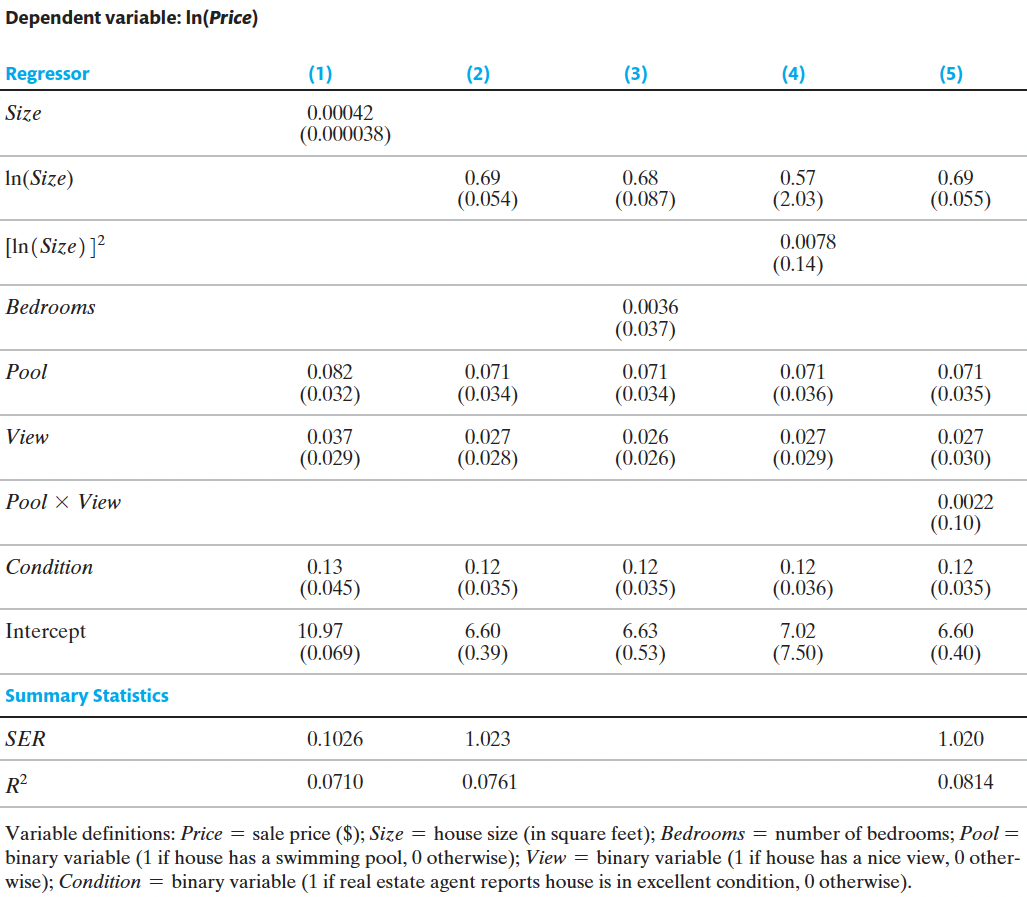
\includegraphics[width=\linewidth]{images/ps4ex3.png}
\end{figure}

\begin{figure}[tbp]
\caption*{Figure 1}
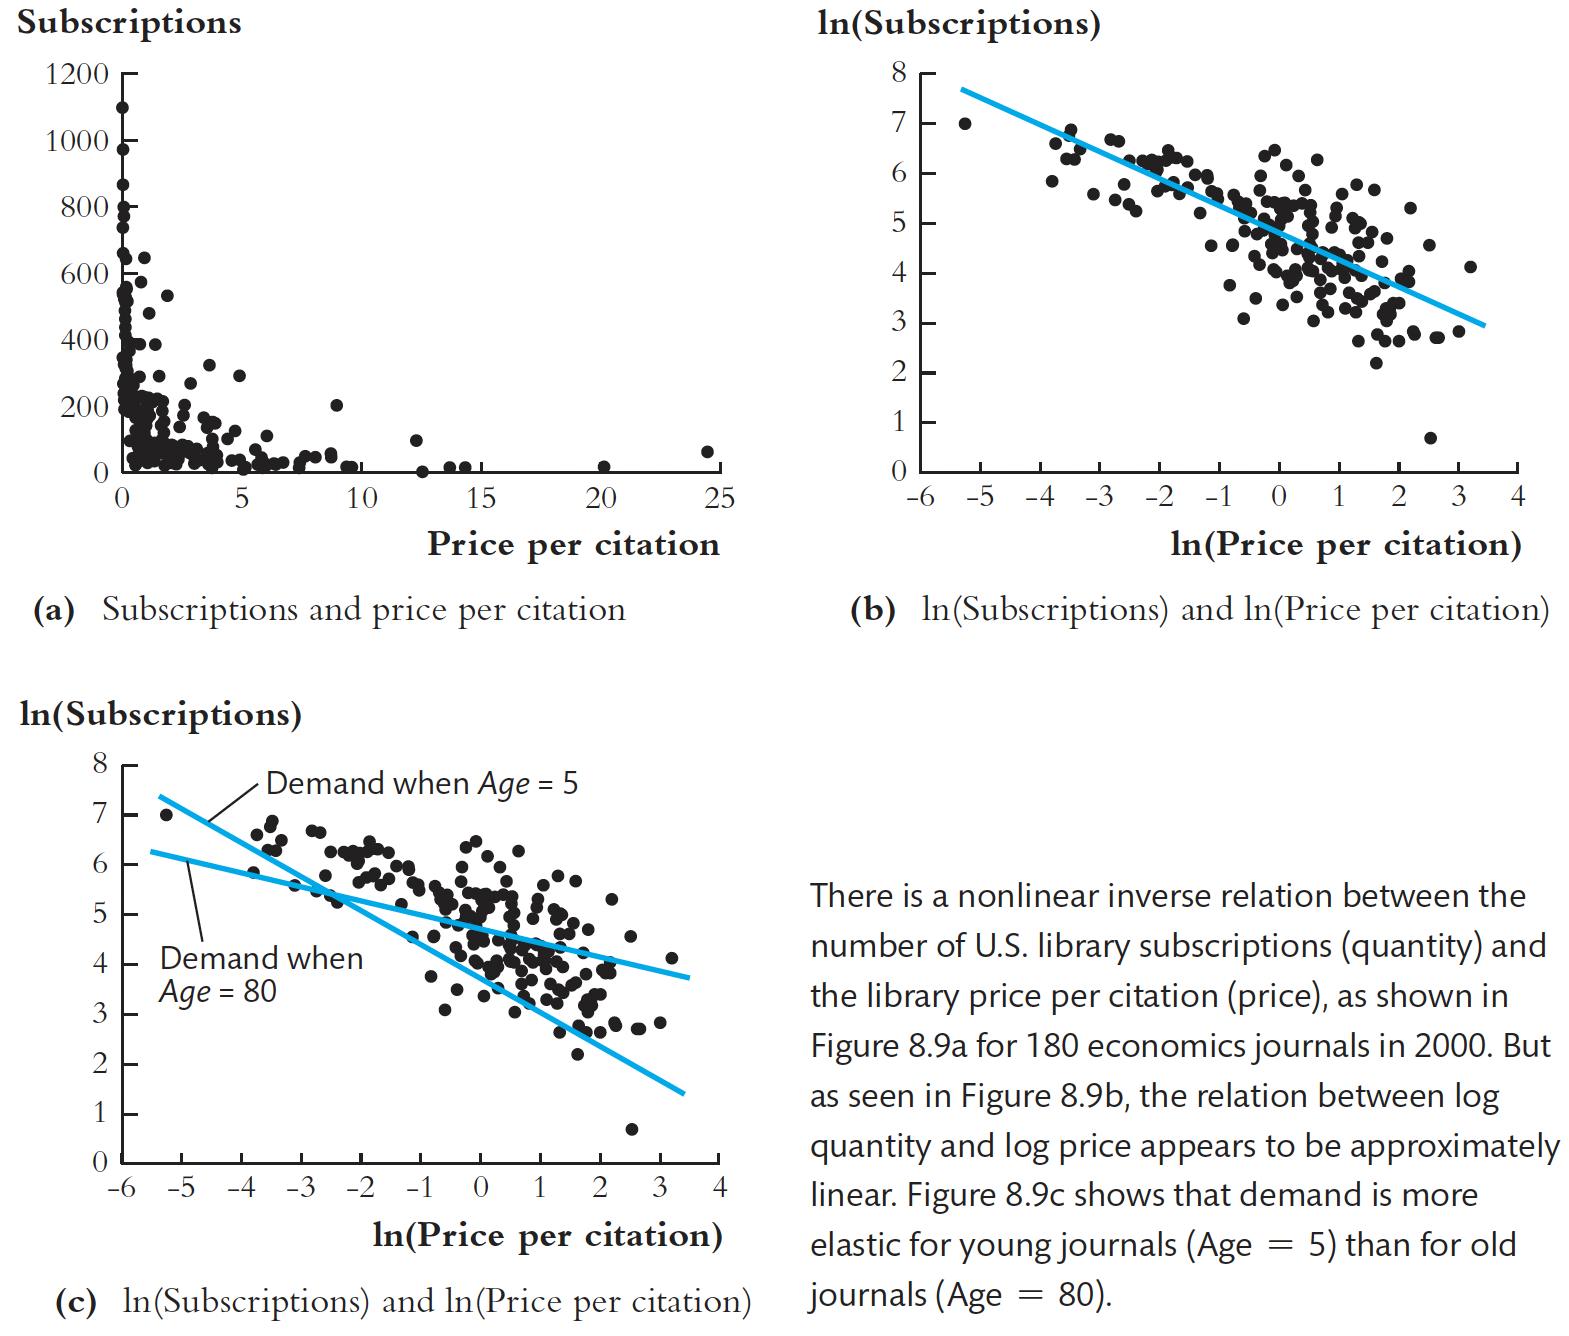
\includegraphics[width=\linewidth]{images/ps4ex4_1.png}
\end{figure}

\begin{figure}[tbp]
\caption*{Table 2}
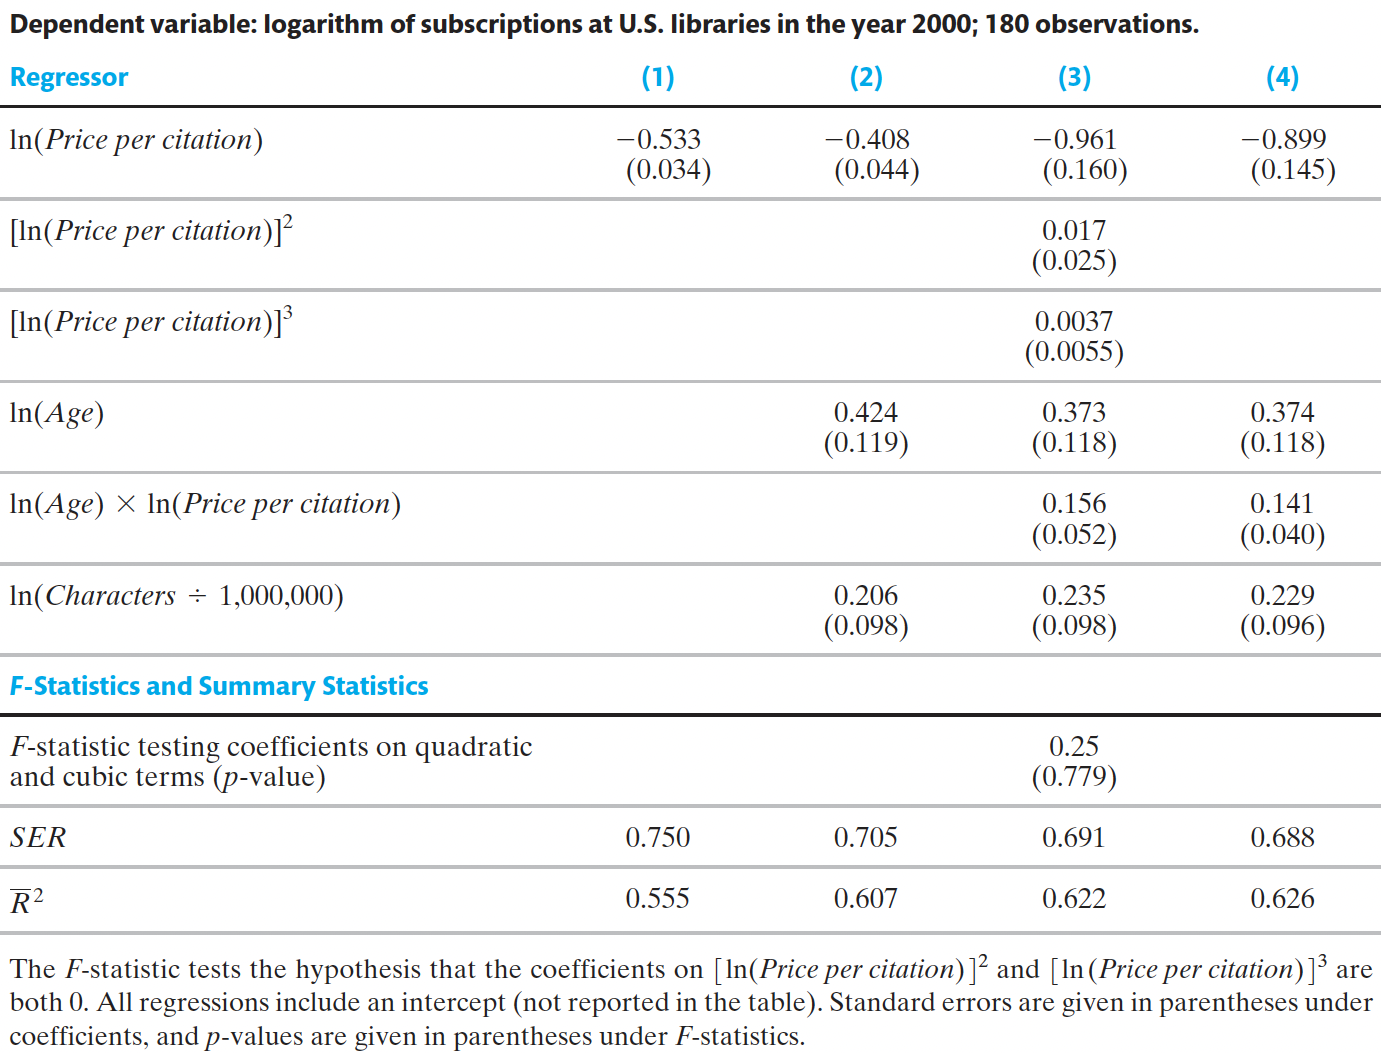
\includegraphics[width=\linewidth]{images/ps4ex4_2.png}
\end{figure}


\end{document}
